\section{Instruções de utilização}
\label{sec:utilizacao}

Para facilitar o entendimento da interface do {\it webscan} podemos
dividi-la em diferente elementos, como mostra a figura \ref{fig:interface}.

\begin{figure}[ht]
\begin{center}
\scalebox{0.55} {
    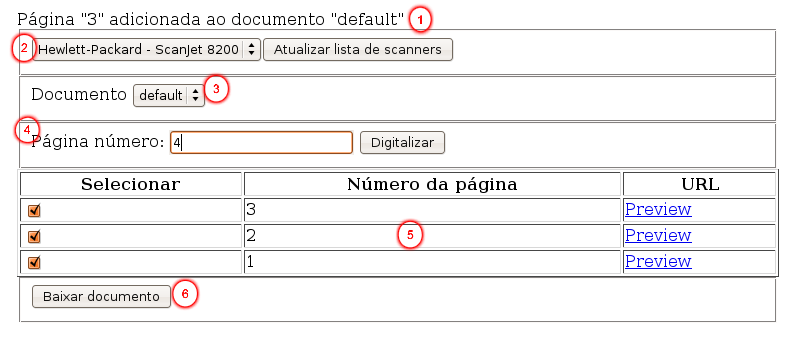
\includegraphics{imagens/interface.png}}
\end{center}
  \caption{Elementos da interface gráfica numerados}
  \label{fig:interface}
\end{figure}

A descrição de cada elemento e respetictivas intruções de uso
serão apresentadas nas seções a seguir.


\subsection{Elemento 1: Área de notificação}
Nesta área serão exibidas todas as mensagens de sucesso e
erro do sistema. Todas as mensagens apresentadas são simples 
e auto-explicativas para que o usuário sempre saiba que 
operação o software esta executando ou qual a razão da tarefa 
solicitada não ter sido atendida.

\subsection{Elemento 2: Lista de scanners disponíveis}
Ao abrir o {\it webscan} a lista de scanners disponíveis no 
momento será atualizada automaticamente. Para atualizar a 
lista novamente basta pressionar o botão "Atualizar lista 
de scanners".

Scanners que estão sendo utilizados não serão listados aqui. 

\subsection{Elemento 3: Lista de documentos}
Esta lista apresenta todos os documentos que contém ao menos
uma página digitalizada. 

Para criar um novo documento selecione a opção "Novo documento"
e digite o nome desejado para o documento na caixa de texto
que aparecerá ao lado da lista. O novo documento será criado
apenas após a digitalização da página. 

\subsection{Elemento 4: Número da página}
O número da página tem duas finalidades: dar nome a página digitalizada e
ordenar as páginas do documento gerado.

Para digitalizar uma página selecione um documento, escolha o número da 
página e pressione o botão "Digitalizar". Durante e após a digitalização
são exibidas mensagens informativas na área de notificação.

Caso o número da página escolhido já exista a página não será digitalizada
e uma mensagem informando o que ocorreu será apresentada na área de 
notificação.

\subsection{Elemento 5: Páginas do documento}
Ao selecionar um documento todas as páginas já digitalizadas pertencentes a
ele serão exibidas nesta tabela. Para utilizar a página no documento PDF que
será gerado basta mante-la selecionada (coluna "Selecionar") como mostra a 
figura \ref{fig:interface}.

Para visualizar a página digitalizada basta clicar no link "Preview" da página
desejada.

\subsection{Elemento 6: Baixar documento}
Este botão gera um documento PDF com todas as páginas selecionadas do 
documento escolhido. O documento gerado ficará disponível para download 
imediatamente.





